\documentclass[12pt]{iopart}
\usepackage{bm}
\usepackage{graphicx}

\def\S{\hat{S}}
\def\W{\hat{W}}
\def\C{\hat{C}}
\def\f{\hat{f}}
\def\g{\hat{g}}
\def\h{\hat{h}}
\def\psii{\bm\psi}
\def\L{\hat{L}}
\def\lmbd{\bm{\lambda}}

\begin{document}
\title[Effective Stokes diagram, symmetries and functional equations for Stokes constants]{Effective Stokes diagram, symmetry relations and functional equations for Stokes constants}
\author{Anton Kutlin}

\address{Institute of Applied Physics of Russian Academy of Sciences, 46 Ulyanov str., 603950 Nizhny Novgorod, Russia}
\ead{anton.kutlin@gmail.com}


\date{\today}

\begin{abstract}
We consider an arbitrary ordinary linear differential equation of the second order and study how its symmetries affect the Stokes constants associated with its general solution. We reformulate the well-known Heading's rules for analytical continuation in a matrix form and propose a concept of an effective Stokes diagram. We show that each two effective Stokes domains which can be overlaid by a symmetry transformation are associated with the same effective Stokes constant and can be described by the same analytical function of a given problem`s parameters evaluated in different points of the parameters` space. We also propose a way to write functional equations for the effective Stokes constants using the equation`s symmetries. This work also contains an example of possible usage of the derived symmetry relations in a case of a real physical problem. 
\end{abstract}

\pacs{02.30.Hq,02.30.Mv}
\submitto{\jpa}

\noindent{\it Keywords\/}:effective Stokes diagram, symmetry, functional equations

%\maketitle

\section{Introduction \label{sec:intro}}
Every linear second-order ordinary differential equation can be put in a form of the stationary one-dimensional Schr\"odinger equation
\begin{eqnarray}
\frac{\rmd^2 y(z)}{\rmd z^2} + Q(z,\lmbd)y(z) = 0,   \label{eq:gen}
\end{eqnarray}
where \mbox{$Q(z,\lmbd)$} will be referred to as a potential. For example, in case of a stationary quantum harmonic oscillator \mbox{$Q(z,E)=E-z^2$}. Briefly, the WKBJ (and often simply WKB) 
approximate solutions of \eref{eq:gen}, so named after
Wentzel, Kramers, Brillouin, and Jeffreys\cite{wkbj}, take the form
\begin{eqnarray}
y_\pm = Q^{-1/4} e^{\pm \rmi \int^z Q^{1/2} \rmd z},   \label{eq:wkb}
\end{eqnarray}
and provided that
$\left|\frac{\rmd Q}{\rmd z}Q^{-3/2}\right| \ll 1 $
a general solution of ~\ref{eq:gen} can be approximated by
\begin{eqnarray}
y = c_+y_+ + c_-y_-.    \label{eq:gensol}
\end{eqnarray}
Clearly, this inequality is not valid in a vicinity of poles or zeros of the potential. Such points will be referred to as singular points and the vicinity of a singularity will be referred to as the interaction area.

%Actually, WKBJ approximation is not the only approximation that can be used for solving ~\ref{eq:gen}. Furthermore, it is not the best. For example, an interesting and effective arbitrary-order approximation generated from unspecified base functions was proposed by Fr\"omans \cite{fromanA,fromanB} – and the only difference between them is that the potential in ~\ref{eq:gen} and $Q$ in
%~\ref{eq:wkb} are not necessarily equal. The range of applicability of the results of this article is not restricted to the WKBJ approximation and extends to any approximation of phase-integral type with the corresponding symmetry properties. This extension can be done by replacement of $\sqrt{Q(z,\lmbd)}$ with an appropriate phase integrand everywhere in the article below. 

The powerful Method of Phase Integrals allows the construction of a globally defined asymptotic expression for the solution of a desired linear ordinary differential using Stokes constants. Unfortunately, there are very few cases when the constants can be found exactly, so approximate methods of different kinds \cite{white,ours} are usually used. This is mostly due to a lack of sufficient equations for the Stokes constants. This work proposes a way of reducing the number of independent unknown Stokes constants using symmetries of a given differential equations. We show that frequently different Stokes constants can be described by the same analytical function of a given problem`s parameters evaluated in different points of the parameter space.  We also propose a way to write functional equations for the Stokes constants using the equation`s symmetries. This work also contains an example of possible usage of the derived relations in a case of a real physical problem. 

The Phase Integral Method was first proposed by A.Zwaan in his dissertation in 1929 \cite{zwaan}. He suggested allowing the independent variable in the differential equation to take complex values and to study a behaviour of the asymptotic solution far away from any singularities. According to Stokes\cite{stokes}, for any given exact solution of ~\ref{eq:gen} coefficients $c_+$ and $c_-$ in the approximate solution (~\ref{gensol}) differ from one domain of the complex plane to another. Such abrupt changes happen on the so-called Stokes lines and have a form of a single-parameter linear transform\cite{heading}. This is called the Stokes phenomenon. The parameter associated with a particular Stokes line is called the Stokes constant. Knowing all Stokes constants associated with a particular potential gives the ability to obtain a globally defined approximate solution of ~\ref{eq:gen}\cite{heading,white} and the Method of the Phase Integrals provides a simple way to find these constants and to write the solution. Unfortunately, there are very few cases when the method allows finding all the constants exactly, so approximations of different kinds \cite{white,ours} are commonly used. This happens mostly because of a lack of exact equations for the Stokes constants, and we provide a recipe to reduce the number of independent Stokes constants for a particular problem using different symmetries of ~\ref{eq:gen}.

Usually for any solution`s analytical continuation around an interaction area the Heading`s rules \cite{white} are used. It is convenient for us to transform these rules into matrix form. 
In \sref{sec:mtrxfrm} the matrix formulation of Heading`s rules is given. 
In \sref{sec:smmtrs} the symmetry relations are obtained from simple considerations. 
In \sref{sec:weber} the relations are used to find the exact form of reflection and transmission coefficients for the Weber equation. 
%In section \ref{BLCKHL} the relations are used for a problem with multiple parameters.
And, finally, in \sref{sec:cnclsns} are the conclusions. 

\section{Matrix formulation of the Heading`s rules of analytical continuation \label{sec:mtrxfrm}}
To start with, let's define some basic concepts. At every point $z$ of the complex plane except the singularities we will emphasize two orthogonal directions. Let's define the Stokes direction 
as a direction with $Re \left( \sqrt{Q(z,\lmbd)}dz \right)=0$ and the anti-Stokes direction 
as a direction with $Im \left( \sqrt{Q(z,\lmbd)}dz \right)=0$. We will also use a notion of the Stokes (anti-Stokes) field as a set of Stokes (anti-Stokes) directions for the entire complex plane. Following \cite{heading, white}, we introduce Stokes (anti-Stokes) lines as a paths along Stokes (anti-Stokes) field emanating from the potential`s singularities. Any domain of the complex plane bounded by the Stokes (anti-Stokes) lines and containing no other Stokes (anti-Stokes) lines will be referred to as the anti-Stokes (Stokes) domain. If the potential $Q(z,\lmbd) \sim z^n$ as $z$ goes to complex infinity, then there are $n+2$ Stokes (anti-Stokes) domains in the vicinity of the infinity - we will call such domains the Stokes (anti-Stokes) wedges. Asymptotic phase-integral solutions $y_\pm$ (~\ref{eq:wkb}) oscillate along anti-Stokes lines with equal amplitudes and increase (or decrease) exponentially with constant phase along Stokes lines. The increasing (decreasing) solution will be called dominant (subdominant) in a given Stokes wedge. Strictly speaking, for every point except points of anti-Stokes lines should omit the subdominant solution since otherwise this results in over precision, but we will keep both functions everywhere according to the tradition. For the same reason we will assume, that the Stokes phenomenon occurs strictly on the Stokes line, although it can be detected only by comparing the asymptotic forms of the exact solution on the neighbouring anti-Stokes lines. Also, the complex plane with the potential`s singularities, Stokes and anti-Stokes lines and branch cuts associated with a branching structure of asymptotic solutions (\ref{eq:wkb}) will be referred to as a Stokes plot or diagram. In case of a phase integral approximation different from WKBJ the Stokes diagram as a characteristic of a solution and not an equation must be plotted using an appropriate phase integrand instead of $\sqrt{Q(z,\lmbd)}$.

Heading`s rules of analytical continuation determine how the coefficients $c_\pm$ from ~\ref{gensol} change from one anti-Stokes domain to another. A traditional presentation of these rules can be found in \cite{heading, white}. Here we will introduce a matrix form of the rules for ease of reference.

Let's define a two-dimensional vector space consisting of vectors
\[
\psii= \left(\begin{array}{*{2}{c}} c_+ \\ c_- \end{array}\right).
\]
Then assume that we have two neighbouring anti-Stokes domains $1$ and $2$, and there are corresponding $\psi$-vectors in the domains. Assume also that $y_+$ is dominant in the Stokes domain containing a borderline separating these anti-Stokes domains. In this situation we can relate $\psi_1$ and $\psi_2$ through the Stokes operator $S$ in the following way:
\begin{eqnarray}
\bm\psi_2 = \S(\pm s) \bm\psi_1, \qquad 
\S(\pm s) = \left(\begin{array}{*{2}{c}} 1 & 0 \\ \pm s & 1 \end{array}\right),    
\label{eq:S}
\end{eqnarray}
where $s$ is a Stokes constant. The sign of the Stokes constant as well as its value depends on the chosen base of approximate solutions $y_\pm$ and particularly on the lower limit of integration $z_0$ in the phase integral $\int_{z_0}^z \sqrt{Q(\xi, \lmbd)} \rmd \xi$ - this point will be referred to as a basepoint. We will use a plus sign if we cross the Stokes line in a counterclockwise direction relatively to the basepoint and a minus sign otherwise. If the borderline lies in a Stokes domain where $y_+$ is subdominant we must use $\S^T$ instead of $\S$.

Obviously, $\psii$-vector in a given anti-Stokes domain depends on the chosen basepoint too. As it follows from ~\ref{eq:wkb}, a change of the basepoint from $z_0=a$ to $z_0=b$ in terms of $\psii$-vectors can be written as
\begin{eqnarray}
\psii^{(b)} = \W(b,a) \psii^{(a)}, \qquad 
\W(b,a) =  
\left(\begin{array}{*{2}{c}}
\rme^{\rmi \int_a^b \sqrt{Q(z,\lmbd)} \rmd z} & 0 \\ 0 & \rme^{-\rmi \int_a^b \sqrt{Q(z,\lmbd)} \rmd z} 
\end{array}\right).    \label{eq:W}
\end{eqnarray}
This is analogous to the reconnection formula in the traditional Heading`s form of the continuation rules. In case of a phase integral approximation different from WKBJ $\sqrt{Q(z,\lmbd)}$ must be replaced with an appropriate phase integrand  everywhere in this article. Sometimes we will use the symbol 
$\W(w)=\W(\rmi \int_a^b \sqrt{Q(z,\lmbd)} \rmd z)$ to underline a value of the phase integral. 

Finally, we have to introduce a $\C$-operator associated with crossing a branch cut. Imagine the cut emanating from the potential`s singularity of $k^{th}$ order (positive values of $k$ corresponds to zeros and negative to poles) and place this singularity into the origin. Then assume we want to cross the cut in the positive direction from domain $1$ to domain $2$. Then we have to change our variable from $z$ to $z \rme^{2\rmi\pi}$. Such a change will affect both pre-exponential slow $Q^{-1/4}$ dependency and the phase integral in the exponent of the asymptotic base. Specifically, to implement these changes we have to replace 
$Q^{-1/4}$ by $(-\rmi)^k Q^{-1/4}$ 
and $\int \sqrt{Q(z,\lmbd)} \rmd z$ by $(-1)^k \int \sqrt{Q(z,\lmbd)} \rmd z$. In compact matrix form it can be written as
\begin{eqnarray}
\psii_2 = \C^k \psii_1, \qquad
\C =  \left(\begin{array}{*{2}{c}} 0 & -\rmi \\ -\rmi & 0 \end{array}\right).    \label{eq:C}
\end{eqnarray}
As you can see, the need for the introduction of the $\C$-operator connected with the branching of the asymptotic solutions has nothing to do with a real branching structure of an exact solution. So, keeping in mind this simple rule we will omit any such cuts in the Stokes plot and use cuts only to determine branches of $\sqrt{Q(z,\lmbd)}$ which is necessary for correct definition of phase integrals. 

Now imagine, we have a Stokes domain with several Stokes lines. Crossing this domain means multiple applications of $\S-$ and $\W-$operators, but it is easy to see that only one $\S$ and only one $\W$ can replace every such set of operators always - it follows from the group properties of the upper(lower)-triangular matrices. Consequently, every Stokes domain can be described by only one Stokes constant regardless how many Stokes lines it contains. The difference between this effective Stokes constant and the usual one appears in the limit of well-isolated singularities when the usual Stokes constant approaches its limiting value according to the approximation of isolated singularities while the effective one does not. However, as long as every effective Stokes constant can be expressed in terms of usual Stokes constants and corresponding phase integrals, we can still use the approximation of isolated singularities when we need it. Similarly, every set of anti-Stokes lines going in the same direction can be replaced by only one effective anti-Stokes line. A Stokes diagram consisting of effective Stokes and anti-Stokes lines will be referred to as an effective Stokes diagram. As long as the decision about what group of the Stokes lines can be replaced by an effective one and what cannot depends on the path in the complex plane we chose for our analytical continuation, every differential equation can be described by several effective Stokes plots. Actually, the effective Stokes line can connect any two points of the corresponding Stokes domain if it does not destroy the topology of the entire Stokes diagram, taking into account the specifics of a particular problem. Choosing what points to connect by the effective Stokes line we will indicate what basepoints will be used in a given Stokes domain. One of the advantages of the effective Stokes plot is that it looks much simpler than the usual one - almost every Stokes (anti-Stokes) domain contains only one Stokes (anti-Stokes) line. Another advantage is that we can immediately say how many independent unknowns our problem actually has. 

\section{Symmetries and the corresponding connections between different effective Stokes lines 
\label{sec:smmtrs}}
Let`s define what we mean by a symmetry of a given equation. If we rewrite \eref{eq:gen} in operator form
\begin{eqnarray}
\L(z,\lmbd)[y]=0, \qquad \L(z,\lmbd)=\frac{\rmd^2}{\rmd z^2} + Q(z,\lmbd),   \label{eq:L}
\end{eqnarray}
we can define any ordered set of operators $\{f,g,h\}$ as a symmetry transformation of \eref{eq:L} if
\begin{eqnarray}
\hat{P}_{fgh}L(z,\lmbd)=\f\L(\g z,\h\lmbd)=\L(z,\lmbd)\hat{T}_{fgh},   \label{eq:symdef}
\end{eqnarray}
i.e. if $y(z,\lmbd)$ is a solution of ~\eref{eq:L} then $\hat{T}_{fgh}y(z,\lmbd)$ is another solution and $\hat{P}_{fgh}$ and $\L$ do not have to commute. 
For example, an Airy operator $\L_{Airy}(z) = \frac{\rmd^2}{\rmd z^2} - z$ has two base symmetries: 
$\{\g=\rme^{2 \rmi \pi/3 \hat{e}},\f=\h=\hat{e}\}$ 
and $\{\g=\hat{e},\f=c.c.,\h=c.c.\}$, where $\hat{e}$ is an operator unity and $c.c.$ stands for complex conjugate. The main difference between these two symmetries is that the second one changes a direction of a complex variable`s phase increase and the first one does not. We will refer to the symmetries of the first kind as rotation symmetries and of the second kind as conjugation symmetries. Certainly, both of the symmetries can be discrete and usually are, but it is much more convenient to associate some continuous transformation with it. This can be done by introducing of an auxiliary variable $\mu$ varying from $0$ to $1$ such that, for example, $\g_{cont}(\mu)=1+\mu (\g-1)$, and $\g_{cont}(1)=\g$. As it will be seen from the following discussion the parametrization of the continuous operators can be important for the final result.

\begin{figure}
\centering
\noindent
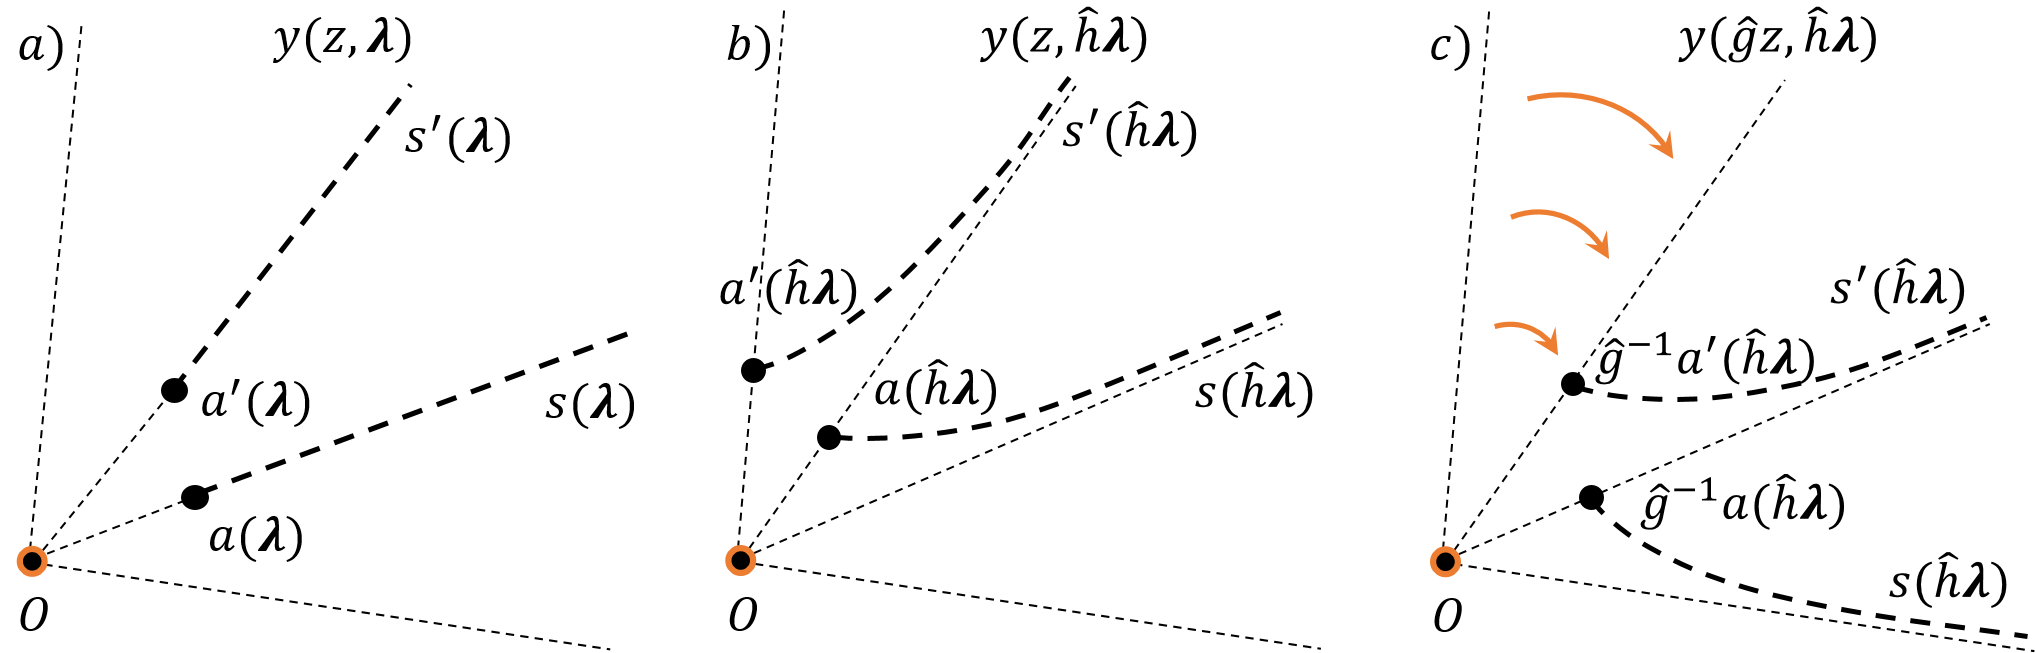
\includegraphics[scale=.5]{stuff/rs.png}
\caption{Stokes diagram`s evolution due to the symmetry transformation}
\label{fig:rst}
\end{figure} 

To understand a consequences of the symmetry`s presence look at \fref{fig:rst}. Every such symmetry transformation can be done in three consecutive steps: transformation of the parameters $\h$, transformation of the independent variable $\g$ and transformation of the whole expression $\f$.   The order of these steps in general matters. As long as the Stokes diagram is a characteristic of a solution and not an equation we will focus on the $\hat{T}_{fgh}$ operator acting on the solution. To be precise, we consider the case when $\hat{T}_{fgh}=\hat{T}_f \hat{T}_g \hat{T}_h$, i.e. the parameters` transformation firstly and the whole expression lastly. The arguments given below can be easily generalized to an arbitrary order.

The operator $\f$ is usually a complex conjugation operator. We will assume here that it can change the value of the Stokes constant but not the structure of the Stokes diagram and that is why it is not necessary to parametrize it. First of all let`s keep track of the basepoints` movement under the continuous parameters` transformation $\h_{cont}(\mu)$. Usually it is convenient to choose some singularity of the potential as a basepoint, but the choice is not necessary for our discussion so we will assume only that it somehow depends on the set of the problem`s parameters $\lmbd$. As long as under this assumption our basepoint $a=a(\h_{cont}(\mu)\lmbd)=a(\mu)$, like the others, is a function of the auxiliary variable $\mu$, the whole Stokes diagram continuously changes preserving its initial topology while  $\mu$ varies from 0 to 1. Assuming also that every Stokes constant is an analytical function of $\lmbd$, we finally arrive at the situation when each transformed Stokes line associates with a new value of the same Stokes constant $s(\h\lmbd)$. The result of this transformation is shown at \fref{fig:rst}.2. Then, we do the same with the independent variable $z$ using $\g_{cont}(\nu)$. Under this transformation the Stokes domains change places and one Stokes line is taken by another one associated with some other Stokes constant $s'(\h\lmbd)$. Due to the symmetry of the problem the final result of these two transformations` composition can differ from the initial configuration only by the basepoints` positions \fref{fig:rst}.3, and that is why $s'(\h\lmbd)$ and $s(\lmbd)$ have to be equally accurate to the corresponding phase integral and the $\f$ transformation. A formal formula expressing this relation is shown below:
\begin{eqnarray}
\fl \S^{(T)} \left( \f s'(\h\lmbd) \right) = 
\W \left( \g^{-1}a'(\h\lmbd),a(\lmbd) \right)
\S^{(T)} \left( s(\lmbd) \right)
\W \left( a(\lmbd), \g^{-1} a'(\h\lmbd) \right).
\label{eq:gensym}
\end{eqnarray}
What to use in the right hand side of \eref{eq:gensym}, $\S$ or $\S^T$, is decided on the basis of general rules from \sref{sec:mtrxfrm}: we use $\S$ for the Stokes domains where $y_+$ is dominant and $\S^T$ otherwise. In the left hand side of \eref{eq:gensym} we have to use the same form as in the right hand side: if the right hand side is an upper(lower)-triangular matrix, then the left hand side is upper(lower)-triangular too. An integration path in the formula can be determined in the following way: we have to decide what path we would use to change a basepoint from $a(\lmbd)$ to $a'(\lmbd)$ and then trace how it deforms under our transformation. And now we can see why and how a resulting symmetry relation can depend on the parametrization of the continuous operators: this dependency is a manifestation of a branching structure of the Stokes constant as a function of the problem`s parameters $\lmbd$.

The relation discussed above allows us to take a fresh look at the nature of the different Stokes constants. Two different Stokes domains which can be overlaid by the transformations $\{\g,\h\}$ are actually associated with the same effective Stokes constant but taken in the different points of the parameters` space. For example, every set of Stokes wedges can be described by only one multidimensional analytical complex function $s(\lmbd)$.

Now let us take a closer look at the important special case of a complex conjugation symmetry. For every potential which does not explicitly include an imaginary unit the symmetry $\f=\g=\h=c.c.$ holds, 
i.e. $\L^*(z^*,\lmbd^*)=\L(z,\lmbd)$ and
\begin{eqnarray}
\S^{(T)} \left( -s'^*(\lmbd^*) \right) = 
\W \left( a'^*(\lmbd^*),a(\lmbd) \right)
\S^{(T)} \left( s(\lmbd) \right)
\W \left( a(\lmbd),a'^*(\lmbd^*) \right).
\label{eq:cnjgtn}
\end{eqnarray}
A minus sign before the Stokes constant in the left hand side of \eref{eq:cnjgtn} is a result of the conjugation symmetry. It appears for any transformation $\g$ which changes the direction of a complex variable`s phase increase (\fref{fig:cst}). Strictly speaking there should be two different general formulas for the rotation and conjugation symmetries, but it is convenient to agree to include this minus sign into the $\f$ operator acting on the Stokes constant.

\begin{figure}
\centering
\noindent
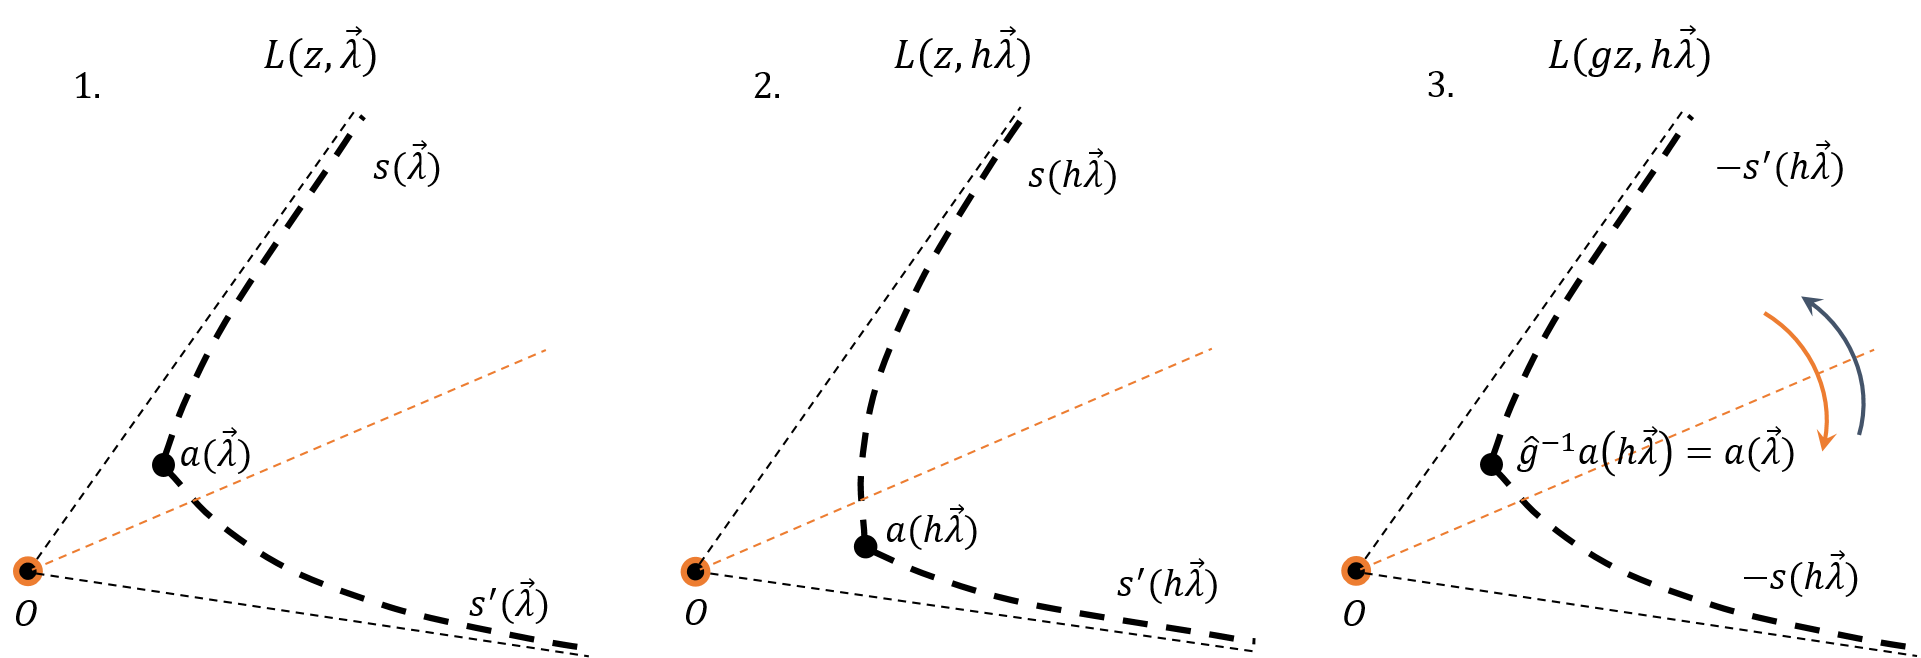
\includegraphics[scale=.5]{stuff/cs.png}
\caption{Stokes diagram`s evolution corresponding to the conjugation symmetry transformation when both conjugate Stokes lines have the same basepoint and $g^{-1}a(h\lmbd)=a(\lmbd)$}
\label{fig:cst}
\end{figure} 

If $a(\lmbd)=a'^*(\lmbd^*)$ as on the \fref{fig:cst}, and $\lmbd$ is real, we obtain a result 
$s^*(\lmbd)=-s'(\lmbd)$ which can be inferred from the symmetry relations presented in \cite{symm}. 
If furthermore $s=s'$ we get an important and extremely simple relation $s^*(\lmbd)=-s(\lmbd)$, i.e. such Stokes constant is purely imaginary providing $\lmbd$ is real.

Another special case of ~\eref{eq:gensym} which is useful to talk about is a case of $\g=\hat{e}$:
\begin{eqnarray}
\S^{(T)} \left( \f s(\h\lmbd) \right) = 
\W \left( a(\h\lmbd),a(\lmbd) \right)
\S^{(T)} \left( s(\lmbd) \right)
\W \left( a(\lmbd),a(\h\lmbd) \right).
\label{eq:func}
\end{eqnarray}
Such case is present for every potential which can be written as a single-valued function of $\lmbd$.
The obtained relation is a functional equation for the considered Stokes constant. Usually such equation helps to illuminate a branching structure of the Stokes constant and write it as a new single-valued function multiplied by the known multivalued one.

\section{Reflection and transmission in the Weber equation \label{sec:weber}}

\begin{figure}
\centering
\noindent
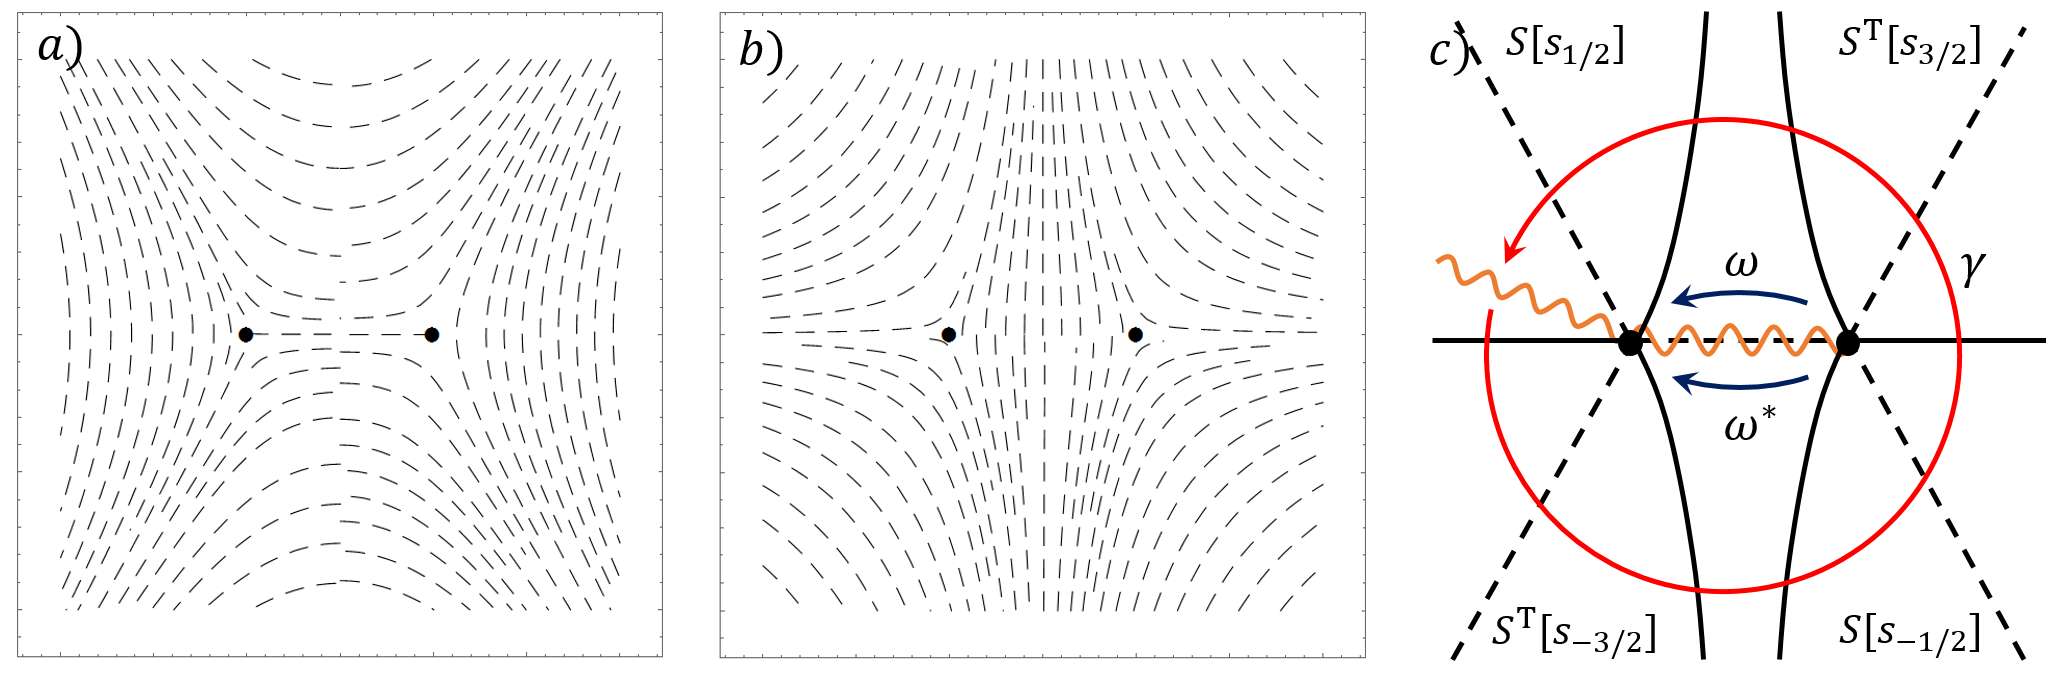
\includegraphics[scale=.5]{stuff/wsd.png}
\caption{Stokes field (1), anti-Stokes field (2) and a Stokes diagram (3) for the Weber equation ~\eref{eq:weber}}
\label{fig:wsd}
\end{figure} 

As an example, consider the Weber equation
\begin{eqnarray}
\frac{\rmd^2 y(z)}{\rmd z^2}+(z^2-\delta^2)y(z)=0
\label{eq:weber}
\end{eqnarray}
with a boundary conditions of a presence of incident wave from the left and absence on such a wave from the right. These conditions can be written using $\psii$-vectors` language as
\begin{eqnarray}
\psii_0 = \left(\begin{array}{*{2}{c}} 1 \\ 0 \end{array}\right),
\label{eq:wbound}
\end{eqnarray}
where $\psii_0$ is a $\psii$-vector in an anti-Stokes wedge containing a ray $Arg(z)=0$. Our aim now is to find scattering characteristics of the solution: a reflection and a transition coefficients. First of all, these characteristics must be written through the Stokes constants. To do it, we must analytically continue our boundary condition (\eref{eq:wbound}) 
to the negative values of $z$. Using \fref{fig:wsd} and the rules from Sec.\sref{sec:mtrxfrm} we write
\begin{eqnarray}
\psii_{\pi} = S[s_{3/2}]W[w]S^T[s_{1/2}]\psi_0 = 
\rme^w \left(\begin{array}{*{2}{c}} 1 \\ s_{3/2} \end{array}\right),
\end{eqnarray}
where $w=\pi\delta^2/2$ is a phase integral calculated above the cut from $z=\delta$ to $z=-\delta$. By the definition the reflection coefficient $R$ is a ratio of the amplitudes of the reflected and incident waves so we have to identify such waves. To do so we must study the phase integral`s behaviour. Since $y_+ \propto e^{i z^2/2}$ hence it is an outgoing wave for $z \rightarrow +\infty$ as well as for $z \rightarrow -\infty$ and
\begin{eqnarray}
R = \frac{1}{s_{3/2}},\ T=i\frac{e^{-w}}{s_{3/2}},
\label{rt}
\end{eqnarray}
where $T$ is a ratio of the amplitudes of the transmitted and incident waves and the imaginary unit arose from the pre-exponential multiplier $Q^{-1/4} \sim x^{-1/2}$.

To find $s_{3/2}$ for the beginning let`s try a traditional method described, for example, in \cite{white}. We can obtain desired equations for the Stokes constants using the single-valuedness of the general solution and analytically continue it around the origin far away from the interaction area:
\begin{eqnarray}
1 = C^2S[s_{3/2}]W[w]S^T[s_{1/2}]S[s_{-1/2}]W[w]S^T[s_{-3/2}],
\label{wgac}
\end{eqnarray}
from which follows
\begin{eqnarray}
\begin{cases} 
s_{1/2} = s_{-3/2}\\
s_{3/2} = s_{-1/2}\\ 
s_{1/2}s_{3/2} + e^{-2w} + 1 = 0
\end{cases}.
\label{webtrad}  
\end{eqnarray}
It is easy to see now that we cannot find $s_{3/2}$ from the system (\ref{webtrad}) - we need at least one more restriction for the Stokes constants. In \cite{white} a requirement of the flux conservation is used and it gives $s_{-1/2}=-s_{1/2}^*$ - it helps to determine $|R|$, but its phase is unknown. Actually the flux conservation is a consequence of the real-valuedness and analyticity of the potential $x^2-\delta^2$ and hence the same relation can be obtained from the conjugation symmetry using ~\ref{cnjgtn}. But it is not the only consequence of the equation`s symmetry, so let`s write them all.

First of all let`s try a rotation symmetry $\{g=e^{i\pi},h=f=1\}$ - it can relate $s_{\pm 3/2}$ with $s_{\mp 1/2}$. Take, for example, $s_{3/2}$ and $s_{-1/2}$. A basepoint of $s_{3/2}$ is chosen to be equal to $-\delta$ on the upper side of the cut and can be written as $b(\delta)=\delta e^{i\pi}$. Obviously, $g^{-1}b(h\delta)=e^{-i\pi}b(\delta)=\delta=a(\delta)$, where $a(\delta)$ is a basepoint of $s_{-1/2}$. According to ~\eref{eq:gensym}, it means that
\begin{eqnarray}
S[s_{3/2}(\delta)] = W[a(\delta),a(\delta)]S[s_{-1/2}(\delta)]W[a(\delta),a(\delta)],
\label{webrs1}
\end{eqnarray}
and
\begin{eqnarray}
s_{3/2} = s_{-1/2}.
\label{webrel1}
\end{eqnarray}
But we have already achieved this result (~\ref{webtrad}) earlier! And it is clear because the corresponding symmetry is just a rotation - it can be seen even from the usual analytical continuation. Similarly, we can obtain $s_{1/2}=s_{-3/2}$, so, the only original equation in the system (\ref{webtrad}) is the last one - it cannot be obtained from any other considerations.

Another rotation symmetry which can relate different Stokes constants is a symmetry $\{g=h=i,f=1\}$ - it can overlaid, for example, 
$s_{1/2}$ and $s_{-1/2}$. Both of the Stokes constants have the same basepoint $a(\delta)=\delta$ 
and $g^{-1}a(h\delta)=(-i)i\delta=\delta$, so
\begin{eqnarray}
S[s_{1/2}(i\delta)] = W[a(\delta),a(\delta)]S[s_{-1/2}(\delta)]W[a(\delta),a(\delta)],
\label{webrs2}
\end{eqnarray}
or
\begin{eqnarray}
s_{1/2}(i\delta) = s_{-1/2}(\delta).
\label{webrel2}
\end{eqnarray}
Considering ~\ref{webrel1} and another analogous relation, we can easily see now that all four Stokes wedges can be described by only one function as was mentioned in the previous section. 

Now let's take a look at the symmetry $\{h=e^{i\pi},g=f=1\}$ - as it was written in the previous section, such a symmetry gives rise to a functional equation which can help to illuminate a branching structure of the Stokes constant. 
For definiteness we will talk about $s_{3/2}$. To understand what to choose as endpoints in the phase integrals in ~\eref{eq:func}, let`s parametrize $h$ as $h_{cont}(\mu)=e^{i\pi\mu}$ and look at ~\ref{wrs}. Obviously, for $s_{3/2}$ a basepoint $a(\delta)=\delta e^{i\pi}$ and the question is how it is changing under our transformation. Using ~\ref{wrs} we see that finally it arrives in $z=\delta$, but the phase matters because it defines a branch of the integrand $\sqrt{Q(z,\delta)}$ and that is why 
$a(h\delta)=\delta e^{2i\pi}$ and
\begin{eqnarray}
S[s_{3/2}(\delta e^{i\pi})] = W[-w]S[s_{3/2}(\delta)]W[w],
\label{webrs3}
\end{eqnarray}
or
\begin{eqnarray}
s_{3/2}(\delta e^{i\pi})=s_{3/2}(\delta)e^{-2w}=s_{3/2}(\delta)e^{-\pi\delta^2}.
\label{webrel3}
\end{eqnarray}
This functional equation can be easily solved by substitution $s_{3/2}=i\delta^{i\delta^2}f(\delta^2)$, where $f(\delta^2)$
is single-valued in a sense $f(x)=f(x e^{2i\pi})$.

\begin{figure}
\centering
\noindent
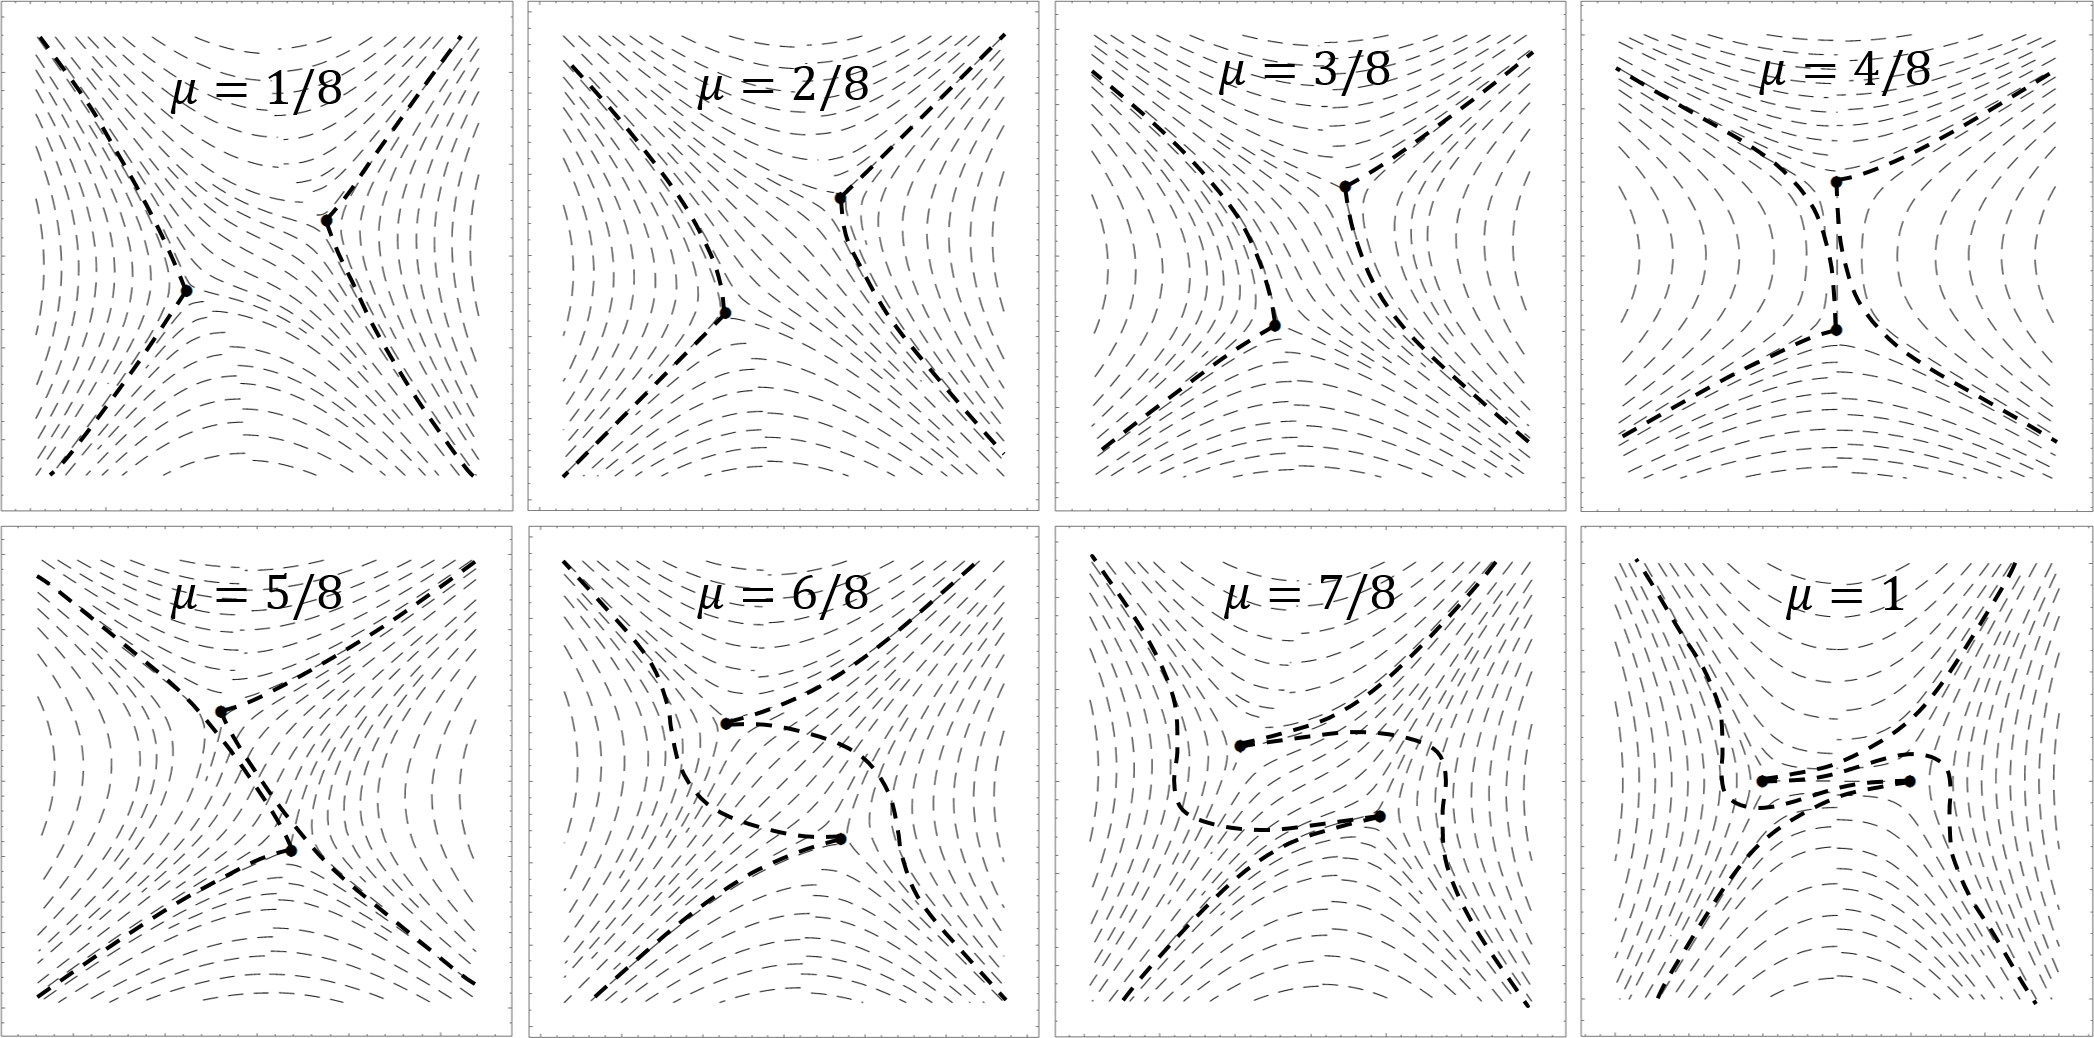
\includegraphics[scale=.5]{stuff/wrs.png}
\caption{Evolution of the Stokes field and effective Stokes lines 
under the continuous parameter`s transformation $h_{cont}(\mu)=e^{i\pi\mu}$}
\label{wrs}
\end{figure} 

And, finally, consider a conjugation symmetry $f=g=h=c.c.$. This symmetry relates the Stokes constants in the upper half plane of the complex plane with the constants in the lower half plane. For example, according to ~\ref{cnjgtn},
\begin{eqnarray}
S[-s_{1/2}^*(\delta^*)] = W[b^*(\delta^*),a(\delta)]S[s_{-1/2}(\delta)]W[a(\lmbd),b^*(\delta^*)],
\label{webcs1}
\end{eqnarray}
and, since $b(\delta)=a(\delta)=\delta$,
\begin{eqnarray}
s_{1/2}^*(\delta^*)=-s_{-1/2}(\delta).
\label{webrel4}
\end{eqnarray}
For real values of $\delta$ ~\ref{webrel4} is nothing but the law of the flux conservation mentioned above. But, for complex values, in conjunction with ~\ref{webrel3} and ~\ref{webrel1} it gives
\begin{eqnarray}
s_{3/2}(\delta)=s_{-1/2}(\delta)=i(i\delta^2)^{i\delta^2/2}p(i\delta^2),
\label{webrel4}
\end{eqnarray}
where $p(x)=p(x e^{2i\pi})$ and $p(x)$ is real on the real axis. Now, using ~\ref{webrel2} and the last equation from the 
system (\ref{webtrad}), we can write a functional equation for $p(x)$:
\begin{eqnarray}
p(x)p(-x)=2cos(\pi x/2).
\label{pfunceq}
\end{eqnarray}
This functional equation is similar to Euler`s reflection formula and can be reduced to it by the substitutions
$x=1-2t$ and $p(x)=u(x)\sqrt{2\pi}/\Gamma(1/2+x/2)$, where $u(x)u(-x)=1$. The function $u(x)$ can be easily found from the boundary conditions for ~\ref{pfunceq}. Indeed, we know exactly \cite{white} that $s(0)=i\sqrt{2}$ and we can assume, according to the approximation of isolated singularities, that every Stokes constant approaches an imaginary unit as $\delta$ goes to plus infinity. Taking into consideration ~\ref{webrel4}, we can say that
\begin{eqnarray}
\begin{cases} 
p(0) = \sqrt{2}\\
p(x) \sim x^{-x/2}\ as\ x \rightarrow \pm i \infty 
\end{cases}.
\label{pbnds}  
\end{eqnarray}
Using also the asymptotics of gamma function, we can finally write that $u(x)=(2e)^{-x/2}$ and
\begin{eqnarray}
s_{3/2}(\delta)=i(i\delta^2)^{i\delta^2/2}\frac{\sqrt{2\pi}(2e)^{-i\delta^2/2}}{\Gamma(1/2+i\delta^2/2)}.
\label{webfinal}  
\end{eqnarray}
This is an exact expression of the Stokes constant for the Weber problem - it can be verified using an exact solution 
of the ~\eref{eq:weber} as it was done in \cite{ours}.
    
%\section{Example 2: two-dimensional parameters` space and a black hole`s lifetime \label{BLCKHL}}

\section{Conclusion \label{CNCLSNS}}

The Method of Phase Integrals is a beautiful and powerful method of differential equations` asymptotic analysis, but its range of applicability is highly restricted to relatively simple tasks. More complicated problems need additional equations for the Stokes constants and that is why different kinds of approximations \cite{white,ours} are usually used. The analysis of the equations` symmetries, presented in this paper, allows the reader to find functional relations between different Stokes constants and thus to reduce the number of unknowns. The main result of the present work is the ~\eref{eq:gensym}. We transformed Heading`s rules \cite{heading,white} into the matrix form to achieve simplicity and automate the procedure of analytical continuation. We also proposed the idea of an effective Stokes diagram which can be a useful tool for simplifying the computations in case of complicated equations. Effective Stokes lines are assumed to be analytical functions with respect to the problem`s parameters and undergo the Stokes phenomenon when the effective Stokes line ceases to coincide with the usual one. We showed that every differential equation has some trivial symmetries which generate nontrivial functional equations for the Stokes constants. The functional equations are likely to be as complex as the initial differential equation but can be used as a measure of the chosen approximation`s accuracy. All the results obtained in the article are valid for the WKBJ approximation as well as for any other approximation of the phase integral type.

It has not escaped the author`s attention that with present day computing the numerically correct solutions are easily obtained, so this result is only of theoretical interest.

%\textbf{Acknowledgement}


\begin{thebibliography}{10}
\bibitem{zwaan} A. Zwaan. Thesis, Utrecht (1929)
\bibitem{fromanA} Fr\"oman, N., and Fr\"oman, P. O., 1974, Ann Phys (NY) 83, 103–107. (Review: Zentralblatt
f¨ur Mathematik und ihre Grenzgebiete, Mathematics Abstracts 279, 190–191, 1974.)
\bibitem{fromanB} Fr\"oman, N., and Fr\"oman, P. O., 1974, Nuovo Cim 20B, 121–132.
\bibitem{wkbj} G. Wentzel, Zeit. f. Phys. 38, 518 (1926), H. A. Kramers,
 Zeit. f. Phys. 39, 828 (1926), L. Brillion, C. R. Acad. Sci. Paris 183, 
24 (1926), H. Jeffries, Philos. Mag. [7] 33, 451 (1942)
\bibitem{stokes} Stokes, G. G., Trans. Camb. Phil. Soc. 10, 105 (1857).
\bibitem{heading} J. Heading. {\it An Introduction to Phase Integral Methods} 
Wiley, NY (1962)
\bibitem{white} R. B. White,
 {\it Asymptotic Analysis of Differential Equations}, Imperial College Press, 2010.
\bibitem{symm} Fr\"oman, N., Fr\"oman, P. O., and Lundborg, B., 1988b, Math Proc Camb Phil Soc 104, 181–191
\bibitem{ours} R.B. White, A.Kutlin {\it Bound state energies using Phase integral methods} 
\end{thebibliography}
\end{document}
